\documentclass{labreport}

% UTF-8 support for Romanian diacritics in code listings
\lstset{style=python,
  literate={ă}{{\v{a}}}1
           {â}{{\^{a}}}1
           {î}{{\^{i}}}1
           {ș}{{\c{s}}}1
           {ț}{{\c{t}}}1
           {Ă}{{\v{A}}}1
           {Â}{{\^{A}}}1
           {Î}{{\^{I}}}1
           {Ș}{{\c{S}}}1
           {Ț}{{\c{T}}}1
}

\begin{document}

% ---------------------------------------------------------
% 1. TITLE PAGE
% ---------------------------------------------------------
\labtitle{1}{Classical Cryptography: Caesar Cipher and Caesar Cipher with Permutation}{Ilie Covali}{gr. FAF-243}{asist. univ. Zaica Maia}

\tableofcontents
\newpage

% ---------------------------------------------------------
% 2. SHORT THEORY
% ---------------------------------------------------------
\section{Short Theory}

\subsection{Introduction to Classical Cryptography}
Classical cryptography primarily relies on two fundamental classes of operations: \textit{transposition} (rearranging the order of plaintext characters) and \textit{substitution} (replacing plaintext characters with alternative symbols, letters, or numbers according to a predetermined rule). 

Monoalphabetic substitution ciphers represent one of the oldest forms of encryption, in which each letter of the plaintext is deterministically replaced by a corresponding letter from a fixed ciphertext alphabet throughout the entire message. In this laboratory work, we investigate two variations of monoalphabetic substitution over the Romanian alphabet: the standard Caesar cipher and the Caesar cipher with a keyword permutation.

\subsection{Alphabet Definition}
The implementations operate on the Romanian alphabet comprising $N = 31$ characters, ordered as follows:
\begin{equation}
\mathcal{A} = [\text{a, ă, â, b, c, d, e, f, g, h, i, î, j, k, l, m, n, o, p, q, r, s, ș, t, ț, u, v, w, x, y, z}]
\end{equation}
Let $I: \mathcal{A} \to \mathbb{Z}_N = \{0, 1, \dots, N-1\}$ be the bijection mapping each character to its zero-based position in $\mathcal{A}$, and let $\mathcal{A}[i]$ denote the character corresponding to index $i \in \mathbb{Z}_N$.

\subsection{The Standard Caesar Cipher}
The Caesar cipher, historically attributed to Julius Caesar, shifts each character of the plaintext forward in the alphabet by a fixed integer key $k$.

\subsubsection{Encryption and Decryption Formulas}
For a plaintext letter $P_i \in \mathcal{A}$ and a numeric key $k \in \mathbb{Z}_N$, encryption is defined by modular addition:
\begin{equation}
C_i = E(P_i, k) = \mathcal{A}\big[(I(P_i) + k) \pmod N\big]
\end{equation}
Decryption performs the inverse operation using modular subtraction:
\begin{equation}
P_i = D(C_i, k) = \mathcal{A}\big[(I(C_i) - k) \pmod N\big]
\end{equation}

\subsubsection{Key Space Analysis}
Because the transformation is entirely governed by the shift parameter $k \pmod N$, any shift of $k \equiv 0 \pmod N$ yields the identity mapping ($C_i = P_i$). Consequently, the set of non-trivial encryption keys is:
\begin{equation}
\mathcal{K}_{\text{Caesar}} = \{1, 2, \dots, N - 1\}
\end{equation}
For the Romanian alphabet with $N = 31$, the key space consists of exactly:
\begin{equation}
|\mathcal{K}_{\text{Caesar}}| = 31 - 1 = 30 \text{ possible keys}
\end{equation}
Due to this minute key space, the Caesar cipher offers negligible computational security. An adversary can perform an exhaustive brute-force search over all 30 keys in microseconds without requiring computational assistance.

\subsection{The Caesar Cipher with Permutation}
The Caesar cipher with a permutation (keyword Caesar cipher) combines a keyword-based permutation of the alphabet with a secondary numeric shift $k$. This addresses a significant structural defect of the standard Caesar cipher: the predictable sequential arrangement of ciphertext letters.

\subsubsection{Building the Permuted Alphabet}
Two secret keys are provided:
\begin{enumerate}
    \item A string keyword $K$ satisfying a minimum length requirement ($\operatorname{length}(K) \ge 7$) and containing characters exclusively from $\mathcal{A}$.
    \item A numeric key $k \in \{1, 2, \dots, N - 1\}$.
\end{enumerate}

The permuted alphabet $\Pi$ of size $N$ is derived as follows:
\begin{enumerate}
    \item \textbf{Deduplication}: Duplicate occurrences of letters in $K$ are eliminated while retaining the initial occurrence order, producing sequence $K' = \operatorname{dedup}(K)$.
    \item \textbf{Alphabet Completion}: The remaining characters from the standard alphabet $\mathcal{A}$ that do not appear in $K'$ are appended in their natural order:
    \begin{equation}
    \Pi = K' \,||\, (\mathcal{A} \setminus K')
    \end{equation}
\end{enumerate}

\subsubsection{Encryption and Decryption Formulas}
Let $I_{\mathcal{A}}(x)$ denote the index of character $x$ in the standard alphabet $\mathcal{A}$, let $\Pi[j]$ denote the $j$-th character of the permuted alphabet $\Pi$, and let $I_{\Pi}(y)$ denote the index of character $y$ within $\Pi$.

For a plaintext character $P_i \in \mathcal{A}$:
\begin{equation}
C_i = E(P_i, k, \Pi) = \Pi\big[(I_{\mathcal{A}}(P_i) + k) \pmod N\big]
\end{equation}
Decryption proceeds by locating the ciphertext character in the permuted alphabet, shifting back by $k$, and retrieving the plaintext character from the standard alphabet:
\begin{equation}
P_i = D(C_i, k, \Pi) = \mathcal{A}\big[(I_{\Pi}(C_i) - k) \pmod N\big]
\end{equation}

\subsubsection{Proof of Invertibility}
Let $m = I_{\mathcal{A}}(P_i)$. The encryption step yields:
\begin{equation}
C_i = \Pi[c], \quad \text{where } c = (m + k) \pmod N
\end{equation}
Since $\Pi$ is a bijective permutation of $\mathcal{A}$, the index of $C_i$ in $\Pi$ is:
\begin{equation}
I_{\Pi}(C_i) = c = (m + k) \pmod N
\end{equation}
Applying the decryption formula:
\begin{align}
(I_{\Pi}(C_i) - k) \pmod N &= \big(((m + k) \pmod N) - k\big) \pmod N \notag \\
&= (m + k - k) \pmod N = m \pmod N = m
\end{align}
Since $\mathcal{A}[m] = P_i$, we obtain $D(E(P_i, k, \Pi), k, \Pi) = P_i$, proving that the cipher is lossless and fully invertible.

\subsubsection{Key Space Analysis}
The theoretical upper bound on any monoalphabetic substitution cipher over $N = 31$ symbols corresponds to the order of the symmetric group $S_{31}$:
\begin{equation}
|S_{31}| = 31! \approx 8.2228 \times 10^{33}
\end{equation}
In the Caesar cipher with permutation, the key space is constrained by the keyword generation process combined with the numeric shift $k \in \{1, \dots, N-1\}$. For a keyword consisting of $m$ unique characters ($7 \le m \le 31$), the number of permutations of length $m$ drawn from $31$ letters is given by the partial permutations $P(31, m) = \frac{31!}{(31-m)!}$.

Taking only the minimum required length $m = 7$:
\begin{equation}
P(31, 7) = \frac{31!}{24!} = 31 \times 30 \times 29 \times 28 \times 27 \times 26 \times 25 = 13,289,628,000 \approx 1.33 \times 10^{10}
\end{equation}
Coupled with the 30 non-trivial numeric shifts, the minimum key space is:
\begin{equation}
|\mathcal{K}_{\text{perm}}| \ge P(31, 7) \times (N - 1) = 1.33 \times 10^{10} \times 30 \approx 3.986 \times 10^{11} \text{ combinations}
\end{equation}
When longer keywords are used, the key space exceeds $10^{15}$ combinations. This renders naive exhaustive search computationally intractable by hand and substantially raises the bar against brute-force attacks compared to standard Caesar. However, because the cipher remains a monoalphabetic substitution, letter frequencies are preserved, meaning the cipher remains vulnerable to statistical cryptanalysis.

\newpage

% ---------------------------------------------------------
% 3. IMPLEMENTATION
% ---------------------------------------------------------
\section{Implementation}

The laboratory tasks were implemented in Python 3 across two dedicated modules: \texttt{caesar1.py} (standard Caesar cipher) and \texttt{caesar2.py} (Caesar cipher with permuted alphabet). Both modules adhere to defensive programming principles, ensuring input sanitization and descriptive error feedback.

\subsection{Alphabet Encoding and Diacritic Handling}
The Romanian alphabet contains five characters with diacritics (\texttt{ă}, \texttt{â}, \texttt{î}, \texttt{ș}, \texttt{ț}). To prevent character corruption and ensure faithful indexing, the alphabet is defined as an explicit UTF-8 list of distinct string characters:

\begin{lstlisting}[style=python]
alphabet = [
    "a", "ă", "â", "b", "c", "d", "e", "f", "g", "h", "i", "î", "j", "k",
    "l", "m", "n", "o", "p", "q", "r", "s", "ș", "t", "ț", "u", "v", "w",
    "x", "y", "z"
]
\end{lstlisting}
\textit{Comment:} The 31 characters are assigned sequential indices from $0$ to $30$. Input text is converted to lowercase upon arrival, preserving whitespace characters to maintain sentence readability.

\subsection{Input Validation Module}
A robust validation layer ensures that only authorized inputs reach the cryptographic core:

\begin{lstlisting}[style=python]
def validate_key(key_input):
    try:
        key = int(key_input)
        if 1 <= key < len(alphabet):
            return key
        else:
            print(f"Error: Invalid key! The numeric key must be an integer between 1 and {len(alphabet) - 1}.")
            return None
    except ValueError:
        print("Error: Invalid key! Key must be an integer number.")
        return None

def validate_text(text):
    if not text:
        print("Error: Input text cannot be empty.")
        return False
    for char in text:
        if char not in alphabet and char != " ":
            print(f"Error: Invalid character '{char}' detected! Only Romanian alphabet letters and spaces are allowed.")
            return False
    return True
\end{lstlisting}
\textit{Comment:} \texttt{validate\_key} verifies that the numeric shift is an integer in the range $[1, 30]$, rejecting out-of-bounds keys and non-numeric inputs. \texttt{validate\_text} iterates through every character, ensuring non-empty input and immediately halting execution if unsupported symbols (e.g. digits or special characters) are detected.

For Task 2, keyword validation verifies both character validity and the minimum length requirement ($\ge 7$ characters):

\begin{lstlisting}[style=python]
def validate_keyword(keyword):
    if len(keyword) < 7:
        print("Error: Keyword is too short! It must be at least 7 characters long.")
        return False
    for char in keyword:
        if char not in alphabet:
            print(f"Error: Invalid character '{char}' in keyword! Only Romanian alphabet letters are allowed (no spaces or numbers).")
            return False
    return True
\end{lstlisting}
\textit{Comment:} Rejects keywords containing fewer than 7 characters or containing non-alphabetic elements, fulfilling the task requirement.

\subsection{Building the Permuted Alphabet}
Task 2 dynamically constructs the substitution alphabet by extracting unique keyword characters and appending the remainder of the original alphabet:

\begin{lstlisting}[style=python]
def build_permuted_alphabet(keyword):
    unique_key = []
    for char in keyword:
        if char not in unique_key:
            unique_key.append(char)
    remaining = [char for char in alphabet if char not in unique_key]
    return unique_key + remaining
\end{lstlisting}
\textit{Comment:} Maintains order of first appearance for keyword characters. The remaining letters of the Romanian alphabet are filtered to avoid duplicates and appended, guaranteeing a bijection of length 31.

\subsection{Encryption and Decryption Routines}

\subsubsection{Task 1: Standard Caesar Cipher}
\begin{lstlisting}[style=python]
def encrypt(text, key):
    result = ""
    for char in text:
        if char in alphabet:
            new_index = (alphabet.index(char) + key) % len(alphabet)
            result += alphabet[new_index]
        else:
            result += char
    print("Encrypted text:", result)
    return result

def decrypt(text, key):
    result = ""
    for char in text:
        if char in alphabet:
            new_index = (alphabet.index(char) - key) % len(alphabet)
            result += alphabet[new_index]
        else:
            result += char
    print("Decrypted text:", result)
    return result
\end{lstlisting}
\textit{Comment:} Performs direct modular rotation $((i \pm k) \pmod{31})$ over the standard alphabet list.

\subsubsection{Task 2: Caesar Cipher with Permutation}
\begin{lstlisting}[style=python]
def encrypt(text, numeric_key, permuted_alphabet):
    result = ""
    for char in text:
        if char in alphabet:
            plain_index = alphabet.index(char)
            cipher_index = (plain_index + numeric_key) % len(alphabet)
            result += permuted_alphabet[cipher_index]
        else:
            result += char
    print("Encrypted text:", result)
    return result

def decrypt(text, numeric_key, permuted_alphabet):
    result = ""
    for char in text:
        if char in permuted_alphabet:
            cipher_index = permuted_alphabet.index(char)
            plain_index = (cipher_index - numeric_key) % len(alphabet)
            result += alphabet[plain_index]
        else:
            result += char
    print("Decrypted text:", result)
    return result
\end{lstlisting}
\textit{Comment:} Encryption looks up the character's position in $\mathcal{A}$, applies the numeric shift $k$, and extracts the symbol from $\Pi$. Decryption locates the ciphertext character in $\Pi$, subtracts $k \pmod{31}$, and recovers the symbol from $\mathcal{A}$.

\newpage

% ---------------------------------------------------------
% 4. RESULTS
% ---------------------------------------------------------
\section{Results}

This section presents the actual execution results of both programs, demonstrating encryption, decryption, and error handling for invalid input conditions.

\subsection{Task 1: Standard Caesar Cipher Execution}

\subsubsection{Encryption Demonstration}
Figure~\ref{fig:caesar1_enc} illustrates the encryption of the plaintext \texttt{"securitatea informatiei"} using numeric shift $k = 5$. The program outputs \texttt{"vîhzumxdxîd msjșurdxmîm"}.

\begin{figure}[H]
    \centering
    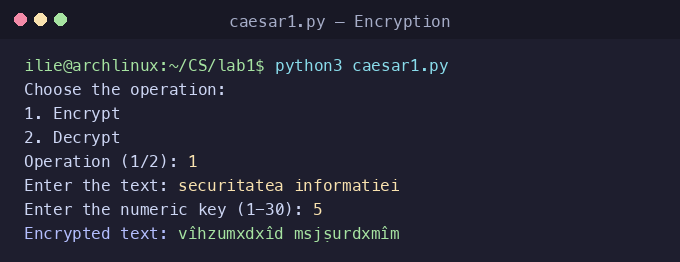
\includegraphics[width=0.88\textwidth]{images/caesar1_encrypt.png}
    \caption{Task 1: Encryption execution using \texttt{caesar1.py} ($k = 5$).}
    \label{fig:caesar1_enc}
\end{figure}

\subsubsection{Decryption Demonstration}
Figure~\ref{fig:caesar1_dec} shows the inverse decryption process. The ciphertext \texttt{"vîhzumxdxîd msjșurdxmîm"} is decrypted with key $k = 5$, correctly recovering \texttt{"securitatea informatiei"}.

\begin{figure}[H]
    \centering
    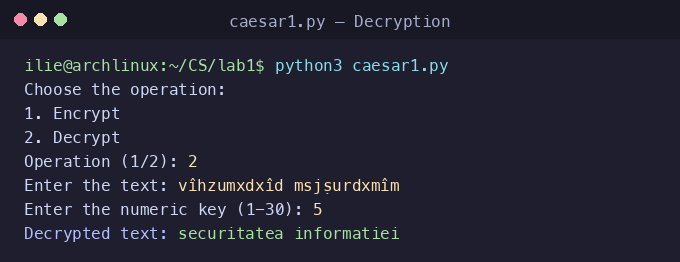
\includegraphics[width=0.88\textwidth]{images/caesar1_decrypt.png}
    \caption{Task 1: Decryption execution using \texttt{caesar1.py} ($k = 5$).}
    \label{fig:caesar1_dec}
\end{figure}

\subsubsection{Input Validation: Out-of-Bounds Key}
When an invalid numeric key outside the range $[1, 30]$ is entered (e.g. $k = 35$), the program detects the error and prints a descriptive error message without terminating abnormally (Figure~\ref{fig:caesar1_inv_key}).

\begin{figure}[H]
    \centering
    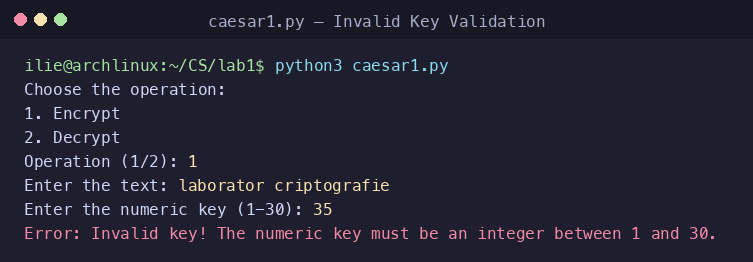
\includegraphics[width=0.88\textwidth]{images/caesar1_invalid_key.png}
    \caption{Task 1: Validation message for an out-of-bounds numeric key ($k = 35$).}
    \label{fig:caesar1_inv_key}
\end{figure}

\subsubsection{Input Validation: Invalid Characters}
Figure~\ref{fig:caesar1_inv_char} displays the result when the user inputs characters not present in the Romanian alphabet (e.g. digits and exclamation mark in \texttt{"parola123!"}).

\begin{figure}[H]
    \centering
    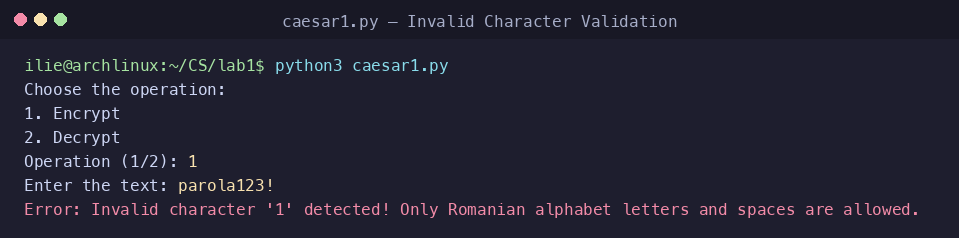
\includegraphics[width=0.88\textwidth]{images/caesar1_invalid_char.png}
    \caption{Task 1: Validation error triggered by invalid characters in plaintext.}
    \label{fig:caesar1_inv_char}
\end{figure}

\newpage
\subsection{Task 2: Caesar Cipher with Permutation Execution}

\subsubsection{Encryption Demonstration}
Figure~\ref{fig:caesar2_enc} depicts encryption under Task 2 using numeric shift $k = 7$ and keyword \texttt{"universitate"}. The program prints both the standard alphabet and the constructed permuted alphabet, encrypting \texttt{"criptografie si securitate"} into \texttt{"bwîșzqgwtfîd xî xdbnwîztzd"}.

\begin{figure}[H]
    \centering
    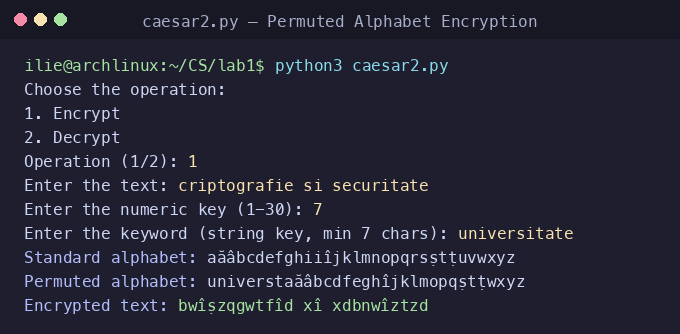
\includegraphics[width=0.88\textwidth]{images/caesar2_encrypt.png}
    \caption{Task 2: Permuted alphabet encryption using \texttt{caesar2.py} ($k = 7, K = \text{"universitate"}$).}
    \label{fig:caesar2_enc}
\end{figure}

\subsubsection{Decryption Demonstration}
Figure~\ref{fig:caesar2_dec} illustrates the decryption of the ciphertext \texttt{"bwîșzqgwtfîd xî xdbnwîztzd"} using the identical key parameters, successfully restoring the original plaintext.

\begin{figure}[H]
    \centering
    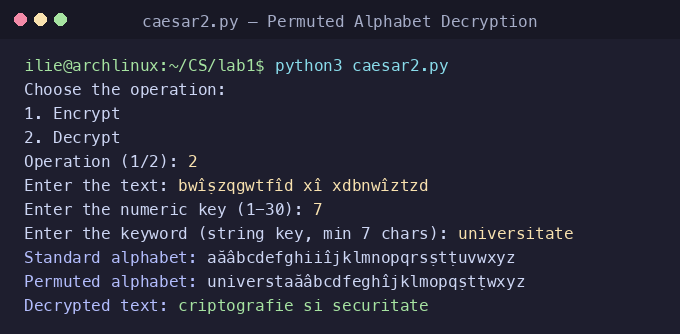
\includegraphics[width=0.88\textwidth]{images/caesar2_decrypt.png}
    \caption{Task 2: Permuted alphabet decryption using \texttt{caesar2.py}.}
    \label{fig:caesar2_dec}
\end{figure}

\subsubsection{Input Validation: Keyword Too Short}
When a keyword with fewer than 7 characters is supplied (e.g. \texttt{"cheie"}, $\operatorname{length} = 5$), the program rejects the input and prompts the user with an explicit error (Figure~\ref{fig:caesar2_short_key}).

\begin{figure}[H]
    \centering
    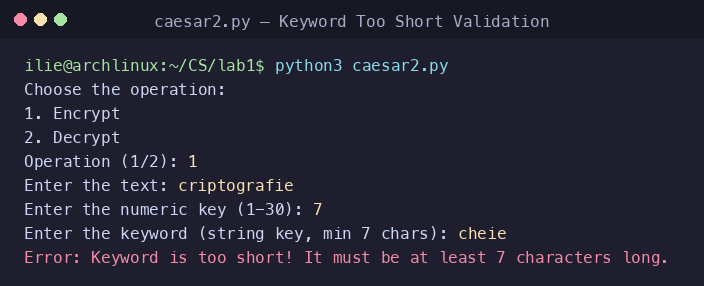
\includegraphics[width=0.88\textwidth]{images/caesar2_short_keyword.png}
    \caption{Task 2: Validation message for a keyword that is too short ($\operatorname{length} < 7$).}
    \label{fig:caesar2_short_key}
\end{figure}

\subsubsection{Input Validation: Invalid Key}
Figure~\ref{fig:caesar2_inv_key} shows the rejection of an invalid shift key $k = 0$, which would otherwise produce a degenerate identity mapping.

\begin{figure}[H]
    \centering
    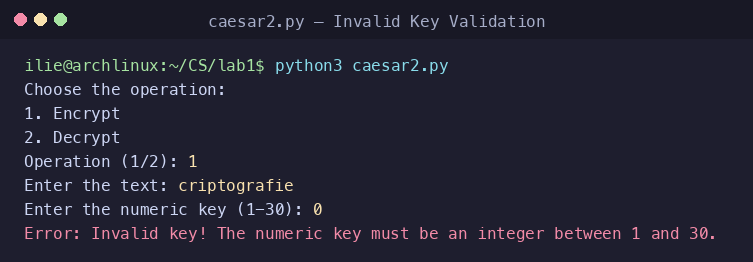
\includegraphics[width=0.88\textwidth]{images/caesar2_invalid_key.png}
    \caption{Task 2: Validation message for an invalid shift key ($k = 0$).}
    \label{fig:caesar2_inv_key}
\end{figure}

\newpage

% ---------------------------------------------------------
% 5. CONCLUSIONS
% ---------------------------------------------------------
\section{Conclusions}

Through the implementation and analysis of the standard Caesar cipher and the Caesar cipher with a keyword permutation, several key cryptographic conclusions can be drawn:

\begin{enumerate}
    \item \textbf{Vulnerability to Brute Force:} The standard Caesar cipher provides zero practical confidentiality. With an effective key space of only $|\mathcal{K}| = 30$ for the Romanian alphabet, an eavesdropper can try all possible keys in seconds. In contrast, introducing a permuted alphabet generated by a keyword of length $\ge 7$ expands the key space to over $3.98 \times 10^{11}$ combinations, rendering manual exhaustive search impossible.
    
    \item \textbf{Persistence of Monoalphabetic Properties:} Despite the massive expansion of the key space in Task 2, both algorithms remain strictly \textit{monoalphabetic substitution ciphers}. Each plaintext symbol maps to exactly one ciphertext symbol for any given key. Consequently, the statistical frequency distribution of the underlying language (such as the high frequency of \texttt{e}, \texttt{a}, and \texttt{i} in Romanian) is preserved in the ciphertext. An attacker with a sufficiently long ciphertext can effortlessly break either cipher using frequency analysis and digram/trigram statistics without ever needing to guess the keyword.
    
    \item \textbf{Importance of Rigorous Input Validation:} In practical cryptographic software, defensive programming is vital. Handling diacritics in UTF-8 encoding, enforcing strict bounds on numeric keys, and rejecting malformed inputs prevent runtime crashes and side-channel leakage.
    
    \item \textbf{Foundational Learning:} This laboratory work provided valuable hands-on experience with modular arithmetic, bijection mappings, permutation generation, and the fundamental dichotomy between key space size and cryptographic security against statistical attacks.
\end{enumerate}

% ---------------------------------------------------------
% 6. SOURCE CODE
% ---------------------------------------------------------
\section{Source Code}

The complete source code for this laboratory work, including both implementations, the report generation scripts, and this \LaTeX{} document, is hosted on GitHub:

\begin{center}
\textbf{GitHub Repository Link:}\\
\url{https://github.com/owhowh0/cs-labs/tree/lab1}
\end{center}

\subsection{Repository File Structure}
The repository contains the following structure:
\begin{itemize}
    \item \texttt{caesar1.py}: Implementation of the standard Caesar cipher with input validation.
    \item \texttt{caesar2.py}: Implementation of the Caesar cipher with keyword permutation.
    \item \texttt{generate\_screenshots.py}: Automation script generating high-resolution terminal execution captures.
    \item \texttt{report/}:
    \begin{itemize}
        \item \texttt{report.tex}: The complete \LaTeX{} source code for this report.
        \item \texttt{labreport.cls}: Custom university report document class.
        \item \texttt{images/}: Screenshot assets documenting program execution.
    \end{itemize}
    \item \texttt{pyproject.toml}: Project metadata and configuration.
\end{itemize}

\end{document}
